% -*- coding: utf-8 -*-

\chapter{自動行動計画問題 (Automated Planning Problem)}
%\chapter{古典的プランニング問題 (Classical Planning Problem)}
\label{ch:classical-planning}

本書の冒頭でグラフ探索アルゴリズムが人工知能のための技術として研究されていると説明した。
人工知能とはさまざまな定義で使われる言葉であるが、グラフ探索は自動推論や自動行動計画のために使うことができるために研究されている。
この章では人工知能の一分野である\define{自動行動計画問題}{automated planning problem}{じどうこうどうけいかくもんだい}について説明する \cite{ghallab:04}。
自動行動計画は初期状態から命題集合で表される目的を達成するための{\bf プラン}を発見する問題である。
自動行動計画のためのモデルは様々提案されている。
最も基本となるモデルは古典的プランニング問題である \cite{fikes:71}。
古典的プランニングは完全情報\footnote{正確には完全情報ではなく、アクションの決定のために必要な情報がすべて得られるという風に定義される。例えば問題に全く関係ない冗長な変数が含まれる場合、その情報がエージェントに与えられない場合を考えることができる。このような問題も冗長な変数を無視し古典的プランニング問題で扱うことができる。}、決定的状態遷移を仮定とするモデルであり、状態空間問題に含まれる \cite{fikes:71}。
古典的プランニングによって様々な実問題を表すことができる。例えばロジスティック\cite{helmert2010scanalyzer,sousa2013toward}、セルアセンブリ\cite{asai2014fully}、遺伝子距離計算\cite{erdem2005genome}、ビデオゲーム\cite{lipovetzky2015a}など、様々な応用問題を含むモデルである。

完全情報、決定的状態遷移の仮定を緩和した問題(確率的モデルや不完全情報モデル)もグラフ探索によって解かれることが多いが、本文の範囲外とする。詳細は詳しい教科書を参照されたい\cite{russelln03}。
なお、プランニング問題はA*などの状態空間探索アルゴリズム以外にも、SATやCSPなどの制約充足問題に変換して解く方法もある \cite{ernst1997automatic,do2001planning}。古典的プランニングのための解法としてはグラフ探索アルゴリズムがstate-of-the-artであるが、例えばマルチエージェント経路探索問題などではSATに変換する手法が効率的であることが知られている \cite{sharon2015conflict}。
%本書は
%これらの面白い議論があるが、本書の範囲外とする\cite{kautz:92}。

\section{定義}
\label{sec:planning-definition}

古典的プランニングは述語論理によって世界が記述される\cite{fikes:71}。
Proposition $AP$は世界の状態において何が真・偽であるかを記述する。
世界の状態はエージェントがアクションを行うことによって遷移し、遷移後の状態は遷移前の状態と異なるpropositionが真・偽でありうる。
古典的プランニングの目的は与えられた初期状態からゴール条件を満たすまでのアクションの列を求めることにある。
以下、定義は\cite{edelkamp:2010:hst:1875144}に従う。

\ddef{古典的プランニング問題、Classical Planning Problem}{
古典的プランニング問題は有限状態空間問題$P = (S,A,s_0,T)$の一つである。
$S \subseteq 2^{AP}$は状態の集合であり、$s_0 \in S$は初期状態、$T \subseteq S$はゴール状態の集合、$A: S \rightarrow S$は可能なアクションの集合である。
}

古典的プランニング問題の最も基本となるSTRIPSモデル\cite{fikes:71}の場合、ゴール条件は命題(proposition)のリストで表せられる$Goal \subseteq AP$。ゴール状態の集合$T$は$p \in Goal$となるすべての$p$が真である状態の集合である。
アクション$a \in A$は適用条件$pre(a)$、効果($add(a)$, $del(a)$)で表せられる。適用条件$pre(a) \subseteq AP$はアクション$a$を実行するために状態が満たすべきpropositionの集合である。効果$add(a)$はアクション$a$を適用後に真になるpropositionの集合であり、$del(a)$は偽になる集合である。
従って、アクション$a$を状態$s$に適用後の状態$s' = suc(s,a)$は
\begin{equation}
	suc(s, a) = (s \cup add(a)) \setminus del(a)
\end{equation}
である。

このようにして、古典的プランニング問題は状態空間問題に帰着することが出来る。
状態空間問題はさらにグラフ探索問題に帰着することができる。
グラフ探索による解法の利点は任意の状態空間問題に対して解法となる点である。
各ドメインに対して特化した手法を用いることなくさまざまな古典的プランニング問題の形式で書ける問題に対して同じグラフ探索の手法が適用できる。
つまりプログラムを使う側に立ってみれば、何かの問題解決を行うにあたって問題の定義のみを与えれば、それをどうやって解くかを考えることなく、問題の解を得ることができるのである。
逆に言えば、効率的なグラフ探索アルゴリズムが開発できれば、あらゆる状態空間問題に対して適用できる汎用な手法が高速化できたと言える。

% TODO: show fast-downward.
プランニングの問題定義やアルゴリズムの実装を見たい方はfast-downward \cite{helmert2006}を見ると良い。
fast-downwardはプランニング問題を解くstate-of-the-artのプランナーである。
本書で紹介するアルゴリズムのほとんどがfast-downwardに組み込まれている。


%なのでグラフ探索アルゴリズムとプランニング研究の大きなテーマの一つとして、どのようにして少ない前提知識から効率的なグラフ探索を行うことができるかが盛んに研究されている。
%具体的には効率的なヒューリスティック関数を自動生成する研究や、並列探索などのハードウエアを利用した方法、あるいは洗練されたデータ構造を利用する方法などが

%As such, a classical planning problem can be solved by an A* search ($G(V', E', w'), s_0', T'$); $V' = S$, $e(v_i, v_j) \in E'$ exists if there exists $a$ such that $v_j = succ(v_i, a)$, $s_0' = s_0$, $T' = T$.

% TODO: PDDLの文字フォントを\textttに
\section{プランニングドメイン記述言語: Planning Domain Definition Language}
\label{sec:pddl}

Planning Domain Definition Language (PDDL) \cite{aeronautiques1998pddl}はプランニング問題を記述されるために用いられる言語の一つである。PDDLはプランニング問題を一階述語論理で表現する。
PDDLはドメイン記述とインスタンス記述の2つに分けられ、Lispのような文法で書かれる。
図\ref{fig:pddl-domain}と図\ref{fig:pddl-instance}はブロックスワールド問題のドメイン記述とインスタンス記述である。
ここでドメインとインスタンスは計算理論などで定義される\define{問題}{problem}{もんだい}と\define{インスタンス}{instance}{インスタンス}に対応する。
ドメイン記述は問いの集合を定義し、インスタンスは一つの問いを指定する。
例えば「グリッド経路探索問題」はドメインであり、そのうちの特定の一つのマップがインスタンスに対応する。
ドメイン記述には\define{述語}{predicate}{じゅつご} (\texttt{predicates})と\define{アクションスキーム}{action scheme}{アクションスキーム} (\texttt{action})がある。
インスタンス記述には\define{オブジェクト}{object}{オブジェクト} (\texttt{objects})と初期状態(\texttt{init})、ゴール状態(\texttt{goal})がある。
これら以外にも例えばオブジェクトの型など様々な文法があるが、簡単のためここでは割愛する。
これらの記述によって古典的プランニング問題が定義される。

まず、命題集合$AP$は述語に含まれる変数にオブジェクトを割り当てることによって得られる。
図の例だと例えば\texttt{(on A B), (on A C), (ontable D),...}などの命題が$AP$に含まれる。
アクション集合$A$はアクションスキームに含まれる変数にオブジェクトを割り当てることによって得られ、アクションの変数は\texttt{parameters}に定義される。
アクション$a$の適用条件$pre(a)$はアクションスキームの\texttt{precondition}にオブジェクトを割り当てることで得られる。\texttt{effect}のうち\texttt{not}のついていない命題は$add(a)$に対応し、\texttt{not}のついた命題は$del(a)$に対応する。
例えばアクション\texttt{(pickup A)}の適用条件は{\texttt{(clear A), (ontable A), (handempty)}}、追加効果は{\texttt{(holding A)}}、削除効果{\texttt{(ontable A), (clear A), (handempty)}}である。
初期状態$s_0$は\texttt{init}の命題集合である。この例では{\texttt{(CLEAR C) (CLEAR A) (CLEAR B) (CLEAR D) (ONTABLE C) (ONTABLE A)}}である。
ゴール条件$Goal$は\texttt{goal}の命題集合である。つまり、ゴール状態集合$T$は$Goal$を含む状態の集合である。

PDDLのミソは一階述語論理によってプランニング問題を記述する点である。
状態空間に含まれる命題を一つ一つ記述するのではなく、述語とオブジェクトの組み合わせによって複数の命題をコンパクトに記述することができる。
また、インスタンス記述を変えることで同じドメインの異なるインスタンスをモデルすることができる。
例えばブロックスワールドのドメイン記述はそのままに、インスタンス記述のオブジェクトや\texttt{init}などを変えることで違う問いにすることができる。

PDDLは状態空間問題だけでなくより広く様々な問題を扱うことができる \cite{aeronautiques1998pddl,fox2003pddl2}。
fast-downwardはPDDLの文法の多くをサポートしているので試してみるには便利である。

\begin{figure}
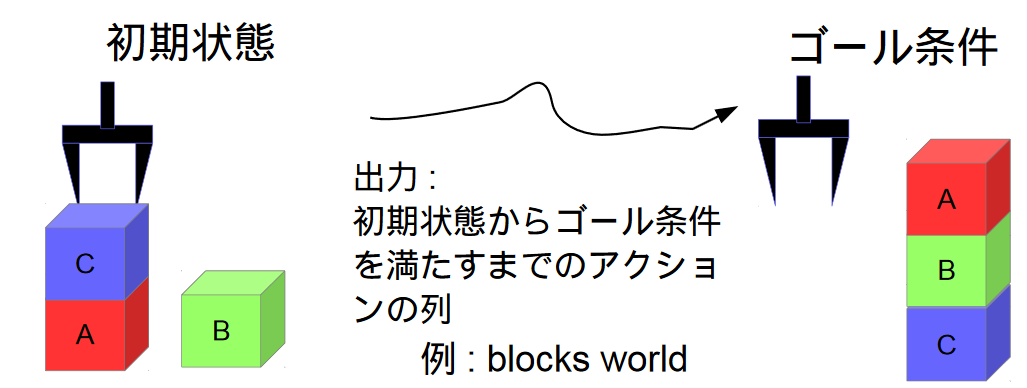
\includegraphics[width=0.8\linewidth]{./figures/blocks-image.png}
\caption{Blocks worldドメイン}
\label{fig:sliding-token}
\end{figure}

\begin{figure}
%\begin{adjustbox}{width=\textwidth,keepaspectratio}
\lstset{language=pddl,basicstyle=\ttfamily\footnotesize,breaklines=true}
\begin{lstlisting}
;;;;;;;;;;;;;;;;;;;;;;;;;;;;;;;;;;;;;;;;
;;; 4 Op-blocks world
;;;;;;;;;;;;;;;;;;;;;;;;;;;;;;;;;;;;;;;;
(define (domain BLOCKS)
  (:requirements :strips)
  (:predicates (on ?x ?y)
	       (ontable ?x)
	       (clear ?x)
	       (handempty)
	       (holding ?x)
	       )

  (:action pick-up
	     :parameters (?x)
	     :precondition (and (clear ?x) (ontable ?x) (handempty))
	     :effect
	     (and (not (ontable ?x))
		   (not (clear ?x))
		   (not (handempty))
		   (holding ?x)))

  (:action put-down
	     :parameters (?x)
	     :precondition (holding ?x)
	     :effect
	     (and (not (holding ?x))
		   (clear ?x)
		   (handempty)
		   (ontable ?x)))
  (:action stack
	     :parameters (?x ?y)
	     :precondition (and (holding ?x) (clear ?y))
	     :effect
	     (and (not (holding ?x))
		   (not (clear ?y))
		   (clear ?x)
		   (handempty)
		   (on ?x ?y)))
  (:action unstack
	     :parameters (?x ?y)
	     :precondition (and (on ?x ?y) (clear ?x) (handempty))
	     :effect
	     (and (holding ?x)
		   (clear ?y)
		   (not (clear ?x))
		   (not (handempty))
		   (not (on ?x ?y)))))
\end{lstlisting}
%\end{adjustbox}
\caption{blocks-worldのdomainファイル}
\label{fig:pddl-domain}
\end{figure}

\begin{figure}
%\begin{adjustbox}{width=\textwidth,keepaspectratio}
\lstset{language=pddl,basicstyle=\ttfamily\footnotesize,breaklines=true}
\begin{lstlisting}
(define (problem BLOCKS-3)
(:domain BLOCKS)
(:objects A B C)
(:INIT (CLEAR C) (CLEAR B) (ONTABLE C) (ONTABLE B)
 (ON C A) (HANDEMPTY))
(:goal (AND (ON A B) (ON B C)))
)

\end{lstlisting}
%\end{adjustbox}
\caption{blocks-worldのinstanceファイル}
\label{fig:pddl-instance}
\end{figure}

\section{古典的プランニング問題の例}
\label{sec:classical-planning-example}

プランニングは様々な問題解決に役立てることができる。
ここでは簡単にプランニングによってどのような問題がモデルできるかを紹介する。

\begin{enumerate}
\item エアポート (airport)
空港の地上の交通管理を行う問題である。
飛行機の離着陸の時間が与えられるのに対し、安全かつ飛行機の飛行時間を最小化する交通を求める問題である。

\item サテライト (sattellite)
人工衛星は与えられた現象を撮影し、地球にデータを送らなければならない。
このドメインはNASAの人工衛星の実際の応用から考案されたものである。

\item ローバー (rovers)
ローバーとは惑星探査ロボットのことである。
この問題は惑星探査ロボットのグループを使って惑星を探索する計画を作る問題である。
ロボットらは興味深い地形などの写真を取るなどの作業を実行する必要がある。
このドメインもNASAの応用をもとにしたものである。

\item パイプスワールド (pipesworld)
複数の原油の油田から複数の目的地にパイプを通して送りたい。
各目的地に定められた量を送るように調整することが目的である。
パイプのネットワークはグラフとしてモデルされており、また同時に原油を通せないパイプの組が存在する。

\item セルアセンブリ (cell assembly)
セルアセンブリは狭いセルの中で働き手が複雑な製品を作成する工場システムである。
大規模な製造ラインと比較して、
セルアセンブリは主に中程度の数(100個程度など)の製品を作るために使われる。
製品の開発や受注生産などに対応して、今生産しなければならない製品を手早く作成するためのセルの行動プランを考えることが問題の目的である。
\cite{asai2014fully}

\item ゲノムリアレンジメント (Genome rearrangement)
ゲノムリアレンジメントは多重整列問題の一つである。
ゲノム間の編集距離とは類似性を測るための指標として使われ、生物の進化の歴史をたどるために使われる。編集距離はあるゲノムから操作を繰り返してもう一方のゲノムに変換するためのコストの総和として定義される。
プランニングモデルを用いることでより様々な操作を定義することができる。例えば遺伝子の位置に入れ替えなど、\ref{sec:msa}節で説明したように単純にグリッド経路探索に落とし込むことのできない複雑な操作を考えることができる。
\cite{erdem2005genome}

\item トラック (trucks)
ロジスティクスと呼ばれる問題の一種である。
トラックを運転してすべての荷物をそれぞれ定められた運び先に届ける問題である。
ただしトラックが運べる荷物の総量は有限であるため、それを考慮して経路を考えなければならない。加えて、届けるまでの期限が存在する荷物が存在する。

\item 工場のセル生産システム

\end{enumerate}

これらの問題はすべて問題に特化した特別なアルゴリズムをそれぞれの問題に対して開発することもできる。多くの場合、特化アルゴリズムの方が汎用プランナーよりも高速である。プランナーの利点は問題に特化した実装をしなくてもPDDLを書くだけで問題を解くことが出来るという点にある。

\section{ヒューリスティック関数の自動生成}
\label{sec:automated-heuristic}

PDDLにはヒューリスティック関数は何を使えばよいかなどの情報は書かれていない。
よって、PDDLを入力とする状態空間問題を解く場合、エージェントはヒューリスティック関数を自動生成しなければならない。
PDDLからヒューリスティック関数を自動生成する手法はプランニング研究の最も重要な研究課題の一つである。

ヒューリスティックの生成方法の一つの指針としては\ref{sec:heuristic-example}節で言及した緩和問題によるヒューリスティックが分かりやすい。
すなわち、元の問題$P$よりも簡単な問題$P'$を生成し、$P$の状態$s$から$P'$の状態$s'$へのふさわしい関数を定義する。そして$h(s)$の値を$P'$における$s'$を初期状態とするゴールへの最適解にする。
このようにしてヒューリスティック関数は自動生成することができる。
以下、具体的にどのような手法があるかを説明する。
各アルゴリズムの実装はfast-downward \footnote{\url{http://www.fast-downward.org}}を参照されたい。

\subsection{ゴールカウントヒューリスティック (Goal Count Heuristic)}

多くの問題ではゴールはいくつかの条件を満たした状態の集合として与えられる。
ゴールカウントヒューリスティックは満たしていないゴール条件の数をヒューリスティック値とする関数である。
例えばスライディングタイルのゴール条件は全てのタイルが所定の位置にあることである。
なので所定の位置にないタイルの数を$h$値とすることが出来る。

ゴールカウントヒューリスティックは許容的であるとは限らない。コスト1のアクションが2つのゴールを同時に満たすかもしれないからだ。1つのアクションで同時に満たせるゴールが1つ以下である場合、そしてその時のみ、許容的である。

\subsection{パターンデータベースヒューリスティック (Pattern Database Heuristic)}
\define{パターンデータベースヒューリスティック}{Pattern database heuristic}{パターンデータベースヒューリスティック}は非常に強力なstate-of-the-artのヒューリスティック関数である\cite{edelkamp2001planning}。
問題の命題集合$AP$に対して$AP' \subset AP$を置き、$AP'$を命題集合とする緩和問題$P'$を考えるというのが大筋の考え方である。
シンプルだが、$AP'$の選び方によっては非常に正確であり、かつ高速なヒューリスティック関数になることが知られている。

% \subsubsection{15パズル}
% パターンデータベースは15パズルのヒューリスティック関数としてよく使われる。
% TODO: 図

\section{関連文献}

複数のパターンデータベースを使ってヒューリスティック値をより正確にすることができる (multiple pattern databases) \cite{holte2004multiple}。
任意の許容的なヒューリスティックの組$h_1, h_2$に対して、$h(s) = max(h_1(s), h_2(s))$は許容的である。このことから、複数のパターンデータベースからヒューリスティック値を計算し、それらの最大値を$h$値とする方法がある。
また、複数のデータベースの$h$値の和$h(s) = h_1(s) + h_2(s)$が許容的なヒューリスティックになる手法もある (disjoint pattern databases) \cite{korf2002}。

パターンデータベースはアブストラクト問題の解を列挙してメモリに保存する。
アブストラクト問題の状態空間の大きさに比例したメモリ量を消費することになる。
それに対して\define{マージアンドシュリンク}{merge and shrink}{マージアンドシュリンク}は複数のアブストラクト問題のグラフをマージして、出来上がったグラフのノードを縮約してグラフを小さくする(シュリンク)手法である \cite{helmert2014merge}。
この方法はパターンデータベースよりもアブストラクト問題を少ないメモリ量で表すことができる。
どのアブストラクト問題をマージするか、どのノードを縮約するかの戦略によってアルゴリズムの性能は大きく変わる。

パターンデータベース、マージアンドシュリンクなどのヒューリスティックはfast downwardに実装されている。興味があれば様々な問題で性能比較をしてみると面白い。

% TODO: landmark cut
%ランドマークカット
%宣言的ヒューリスティック
% Declarative heuristic

